\documentclass[english,11pt]{article}
\usepackage{babel} 
\usepackage[utf8]{inputenc} 			% entree 8 bits iso-latin1
\usepackage[T1]{fontenc}      			% Accents
\usepackage{graphicx}					% Figures (begin{figure})
\usepackage[margin=10pt,font={small,it},labelfont=bf,labelsep=endash,center]{caption}			% Font for caption
\usepackage[a4paper,lmargin=2.5cm,rmargin=2.5cm,tmargin=2.5cm,bmargin=2.5cm]{geometry} 		% Margins
\usepackage[cyr]{aeguill}
%\usepackage[autolanguage]{numprint}		% ecrit les nombre proprement (separation par 10³)  \numprint{1500} 
\usepackage[squaren,Gray]{SIunits}		% SI units    						\unit{\numprint{1500} }{\meter}
\usepackage{url}						% (\url{})
\urlstyle{sf}							% font url
\usepackage[colorlinks=true,linkcolor=black,citecolor=black,urlcolor=black]{hyperref} %\Pour linker des url,
%\usepackage{apalike}					% Biblio style (brackets, do not extend at end of line)
\usepackage{array}						% Pour les tableaux notamment
\usepackage[square]{natbib}				% citep (brackets) et citet (in a sentence)

\graphicspath{{../Figures/}}			% Path to figures
\newcommand{\fig}[1]{(figure~\ref{#1})}
\newcommand{\tab}[1]{(table~\ref{#1})}




\begin{document}
\title{Intrusion of cold waters in the North of the domain. Why AMM60 behaves differently?}
\maketitle

In AMM60, the intrusion of cold water do not extend up to the shelf-break slope current, in winter as well as in summer, whereas in the lower resolution models it reaches up to \unit{61}{\degree N}. Is that due to the slope current, to a different vertical scheme, to something else?
\section{Winter}
\begin{figure}[h!]
	\centering \textbf{WINTER} \\
	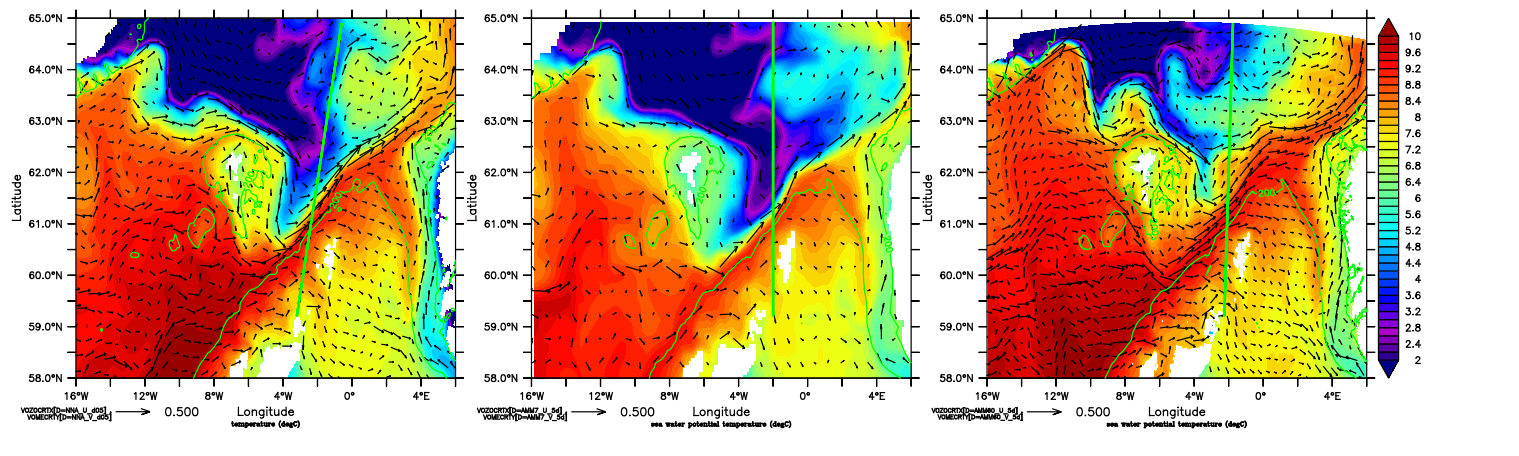
\includegraphics[scale=0.3]{section_2/winter_surface_T_vec_shetland}\\
	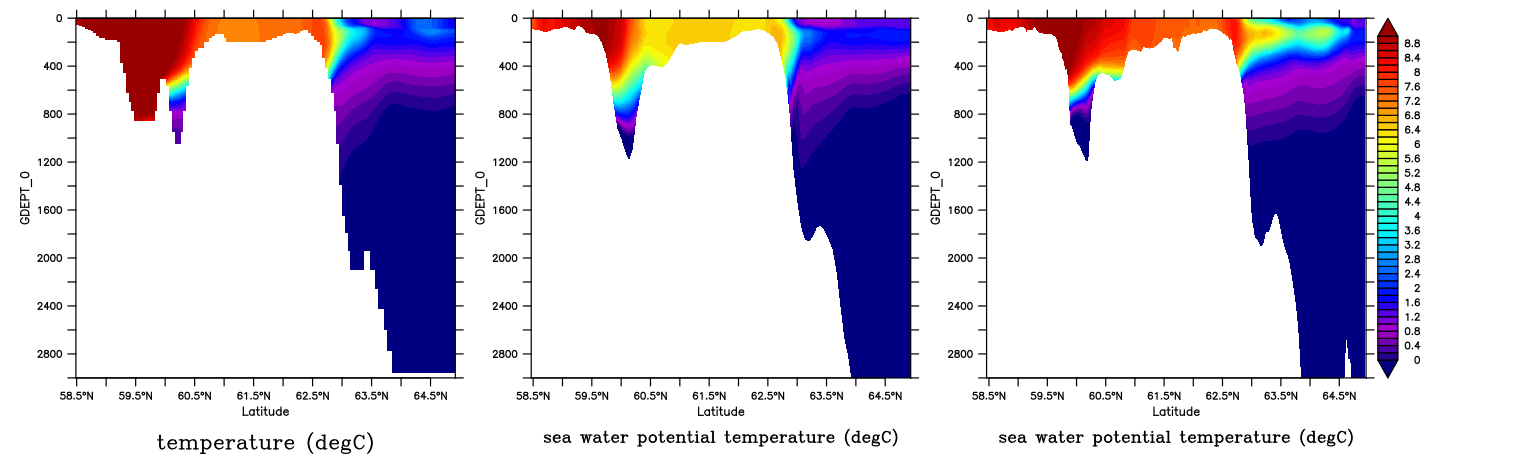
\includegraphics[scale=0.3]{section_2/winter_Section_T_shetland}\\
	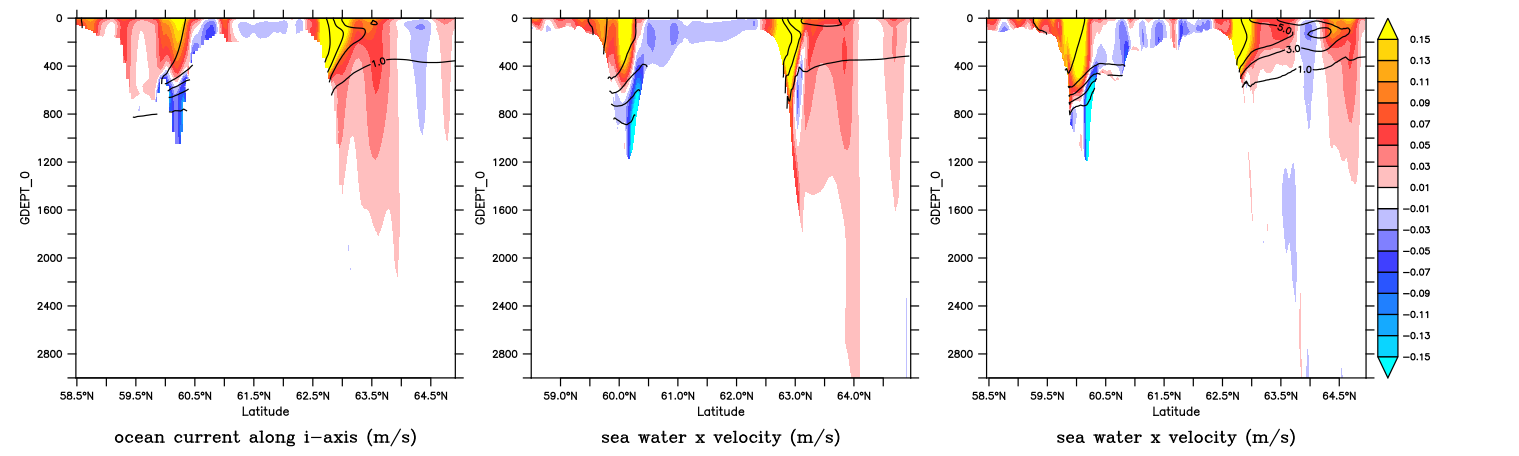
\includegraphics[scale=0.3]{section_2/winter_Section_U_shetland}\\
	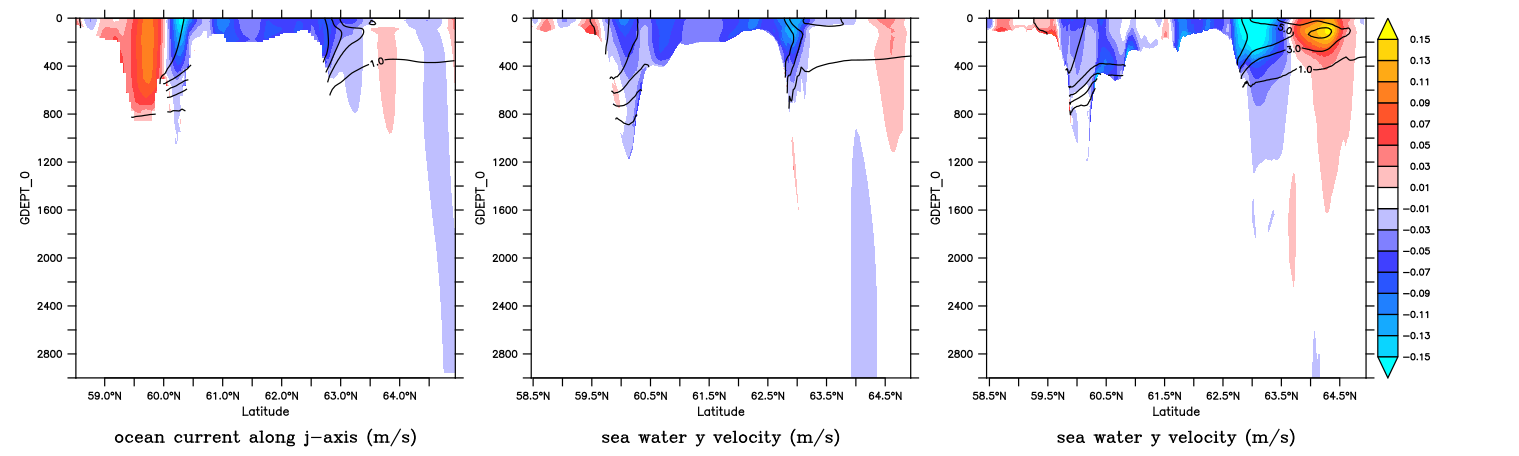
\includegraphics[scale=0.3]{section_2/winter_Section_V_shetland}\\

	\caption{First panel: Surface mean winter temperature and currents for NNA, AMM7 and AMM60 (left to right). Black line shows the location of the vertical section in the following panels.\\ Second to 4th panel: Section of temperature, zonal and meridional velocity at \unit{-6}{\degree E} for NNA, AMM7 and AMM60 (left to right). }
	\label{fig_winter}
\end{figure}

The surface fields of temperature show a warm slope current in all the configuration, blocking the intrusion of cold waters on the shelf \fig{fig_winter}. In AMM60, the patch of cold waters stays north of the Faroe islands (\unit{62.5}{\degree N}), whereas in NNA and AMM7 it reaches up to \unit{61}{\degree N}. 

An eastwards current from Iceland flows along the front in all the configurations, meadering. In AMM60 this current makes more meanders, and warm eddies block the cold flow (e.g \unit{63.2}{\degree N}-\unit{8}{\degree W}, \unit{63.5}{\degree N}-\unit{1.5}{\degree E}). Eddies can also been observed in NNA (e.g. \unit{64}{\degree N}-\unit{0}{\degree E}), but there is less mesoscale activity in AMM7.

If we now look at a latitudinal section east of the Faroe islands: the front of cold waters reaches up to \unit{63}{\degree N} in NNA and AMM7. In AMM60, subsurface warm waters associated with an eddy expand north up to \unit{64.5}{\degree N}. This is associated with a northwards meridional velocity up to \unit{0.15}{\meter\per\second}. No northward meridional velocity is observed on the sections in AMM7 and NNA. Zonal velocities are alike in the 3 configurations, with a westward current along the slope, and an other north of the Faroe islands.

\section{Summer}
The same behaviour is observed in Summer \fig{fig_summer}. The cold path goes as far as \unit{62}{\degree N} in NNA and AMM7, and no more than \unit{64}{\degree N} in AMM60. 
The slope current is still present, and a big eddy is observed at \unit{64}{\degree N}-\unit{11}{\degree W} in all the configurations, limiting the cold inflow on the Icelandic region. The eastwards current from Iceland that we observed in winter is weaker in NNA and AMM7 but still present. In AMM60, it once again is associated with eddies and meanders which completely block the inflow of cold waters.

At the section at \unit{6}{\degree W}, vertical temperatures once again show an extension of warm subsurface water towards the North in AMM60.  These are associated with a complex zonal velocities fields, due to a strong eddy activity.

\begin{figure}[h!]
	\centering \textbf{SUMMER}\\
	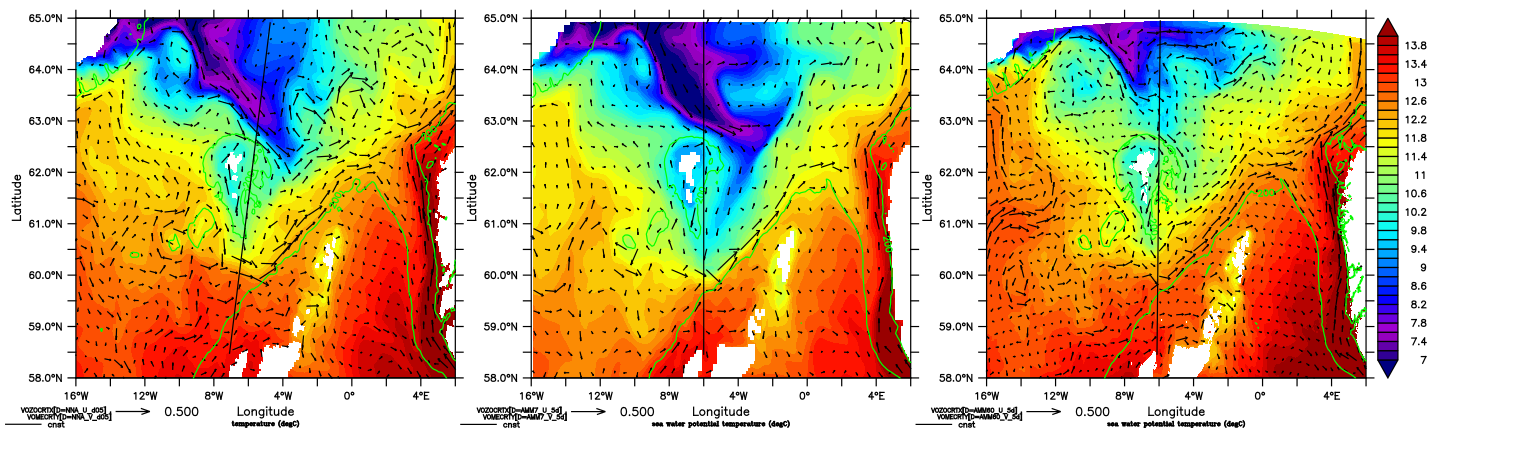
\includegraphics[scale=0.3]{section_2/summer_surface_T_vec_shetland}\\
	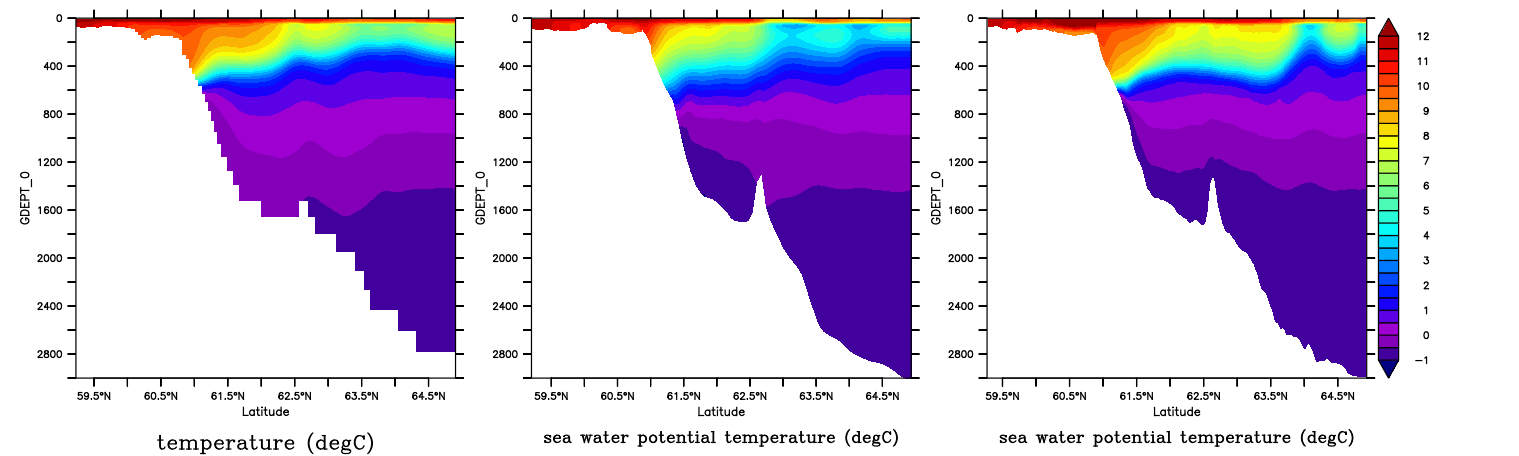
\includegraphics[scale=0.3]{section_2/summer_Section_T_shetland}\\
	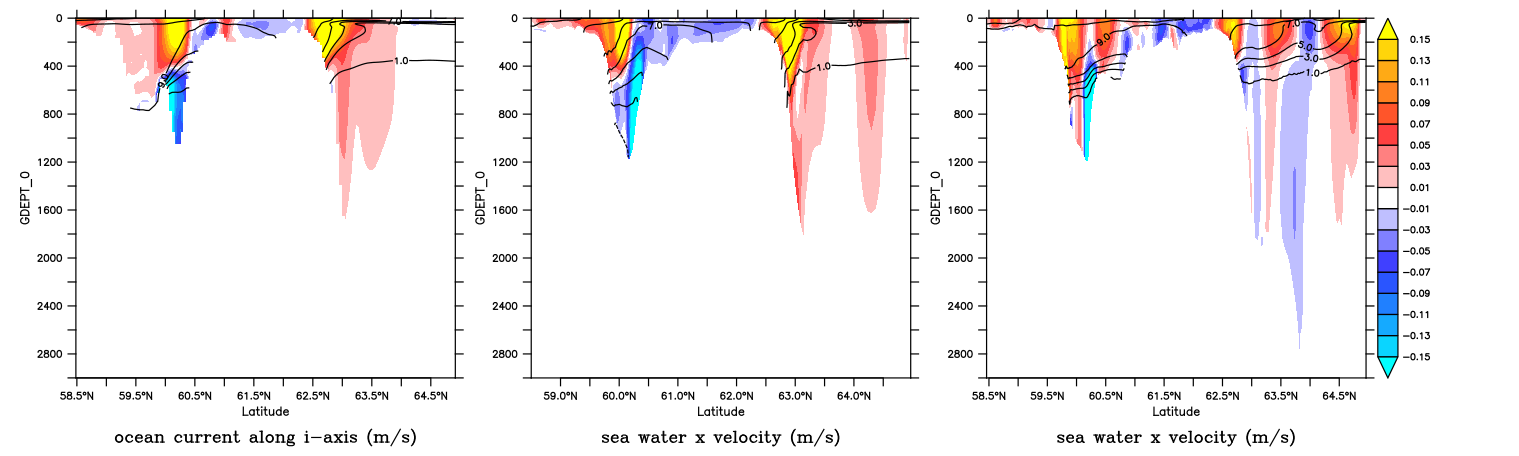
\includegraphics[scale=0.3]{section_2/summer_Section_U_shetland}\\
	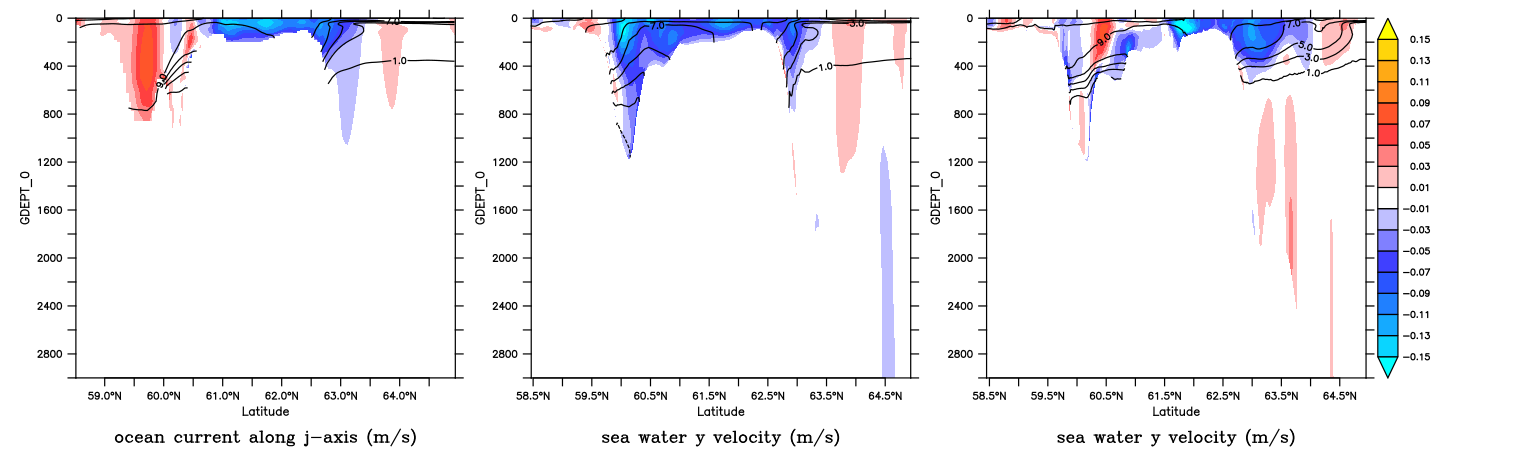
\includegraphics[scale=0.3]{section_2/summer_Section_V_shetland}\\

	\caption{First panel: Surface mean summer temperature and currents for NNA, AMM7 and AMM60 (left to right). Black line shows the location of the vertical section in the following panels.\\ Second to 4th panel: Section of temperature, zonal and meridional velocity at \unit{-6}{\degree E} for NNA, AMM7 and AMM60 (left to right). }
	\label{fig_summer}
\end{figure}



\end{document}